% Appendix A

\chapter{Installation of OpenWRT and TR-069} % Main appendix title

\label{AppendixA} % For referencing this appendix elsewhere, use \ref{AppendixA}

\lhead{Appendix A. \emph{Installation of OpenWRT and TR-069}} % This is for the header on each page - perhaps a shortened title

\lstdefinestyle{DOS}
{
    backgroundcolor=\color{black},
    basicstyle=\scriptsize\color{white}\ttfamily
    numbers=none,
    numbersep=8pt,                   % how far the line-numbers are from the code
    numberstyle=\tiny\color{white}, % the style that is used for the line-numbers
    stepnumber=1                    % the step between two line-numbers. If it's 1, each line will be numbered
}
%----------------------------------------------------------------------------------------
\lstdefinestyle{C}
{
  morekeywords={export}
}
%----------------------------------------------------------------------------------------
This appendix will introduce how to getting and building OpenWRT toolchain, compile TR-069 Client and run the client on the Homelive Box.
%----------------------------------------------------------------------------------------
\section{Getting and building OpenWRT toolchain}

\subsection{Get OpenWRT Source}
First to do is create your OpenWRT folder and get the source code of OpenWRT using git or SVN:
\begin{lstlisting}[style=DOS][language=bash]
  $ tsocks svn co -r44360 svn://svn.openwrt.org/openwrt/trunk/ OpenWRT
\end{lstlisting}
or
\begin{lstlisting}[style=DOS][language=bash]
  $ tsocks git clone git://git.openwrt.org/openwrt.git
\end{lstlisting}

We choose the specific version 44360 because OpenWRT added unsupported libraries after this.

\subsection{OpenWRT Buildroot Configuration}
Then is to run configure interface to personalize your OpenWRT image:
\begin{lstlisting}[style=DOS][language=bash]
  $ make menuconfig
\end{lstlisting}

It will show a interface like below:
\begin{figure}[htbp]
	\centering
		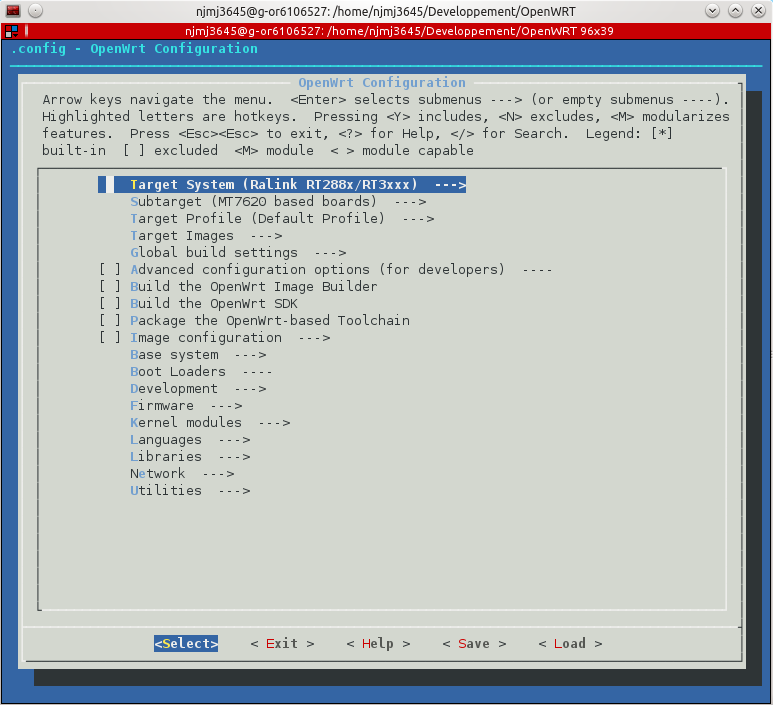
\includegraphics[width=8cm]{Figures/menuconfig.png}
	\caption[OpenWRT Menu Config Interface]{OpenWRT Menu Config Interface}
\end{figure}

\begin{itemize}
  \item In the \textbf{Target System} section, select \textbf{Ralink RT288x/RT3xxx},
  \item In the \textbf{Subtarget} section, select \textbf{MT7620 base boards}.
  \item In the \textbf{Libraries} section, select \textbf{libcurl}.
  \item In the \textbf{Libraries/SSL} section, select \textbf{libopenssl}.
  \item In the \textbf{Base system} section, select \textbf{lipthread}.
\end{itemize}

Then save the new configuration and exit menuconfig.


\subsection{Build the OpenWRT Toolchain}
\begin{lstlisting}[style=DOS][language=bash]
  $ tsocks make
\end{lstlisting}
If there are errors during the compilation. After solving the problem, you can continue the compilation process by using commands like:
\begin{lstlisting}[style=DOS][language=bash]
  $ tsocks make package/install
\end{lstlisting}
or
\begin{lstlisting}[style=DOS][language=bash]
  $ tsocks make package/libs/curl/install
\end{lstlisting}

The compiling process may take a while. When finished, your OpenWRT toolchain is ready to use.

%----------------------------------------------------------------------------------------
\section{Building TR-069 Client}
\subsection{Get the source code}
Getting the source code by using the SVN of Orange:
\begin{lstlisting}[style=DOS][language=bash]
  $ tsocks svn co https://www.forge,orange-labs.fr/svnroot/tr069agent
\end{lstlisting}


Before using OpenWRT toolchain, there are some path to set:
\begin{lstlisting}[style=DOS][language=bash]
  $ export STAGING_DIR=$HOME/path/to/openwrt/staging_dir
  $ export PATH=$PATH:$STAGING_DIR/toolchain-mipsel_24krec+dsp_gcc-4.8-linaro_uClibc-0.9.33.2/bin
\end{lstlisting}

Then, the compiling command is:
\begin{lstlisting}[style=DOS][language=bash]
  $ make Target=HomeLive CC=$STAGING_DIR/toolchain-mipsel_24kec+dsp_gcc-4.8-linaro_uClibc-0.9.33.2/bin/mipsel-openwrt-linux-uclibc-gcc CWMP_APPLICATION_NAME=cwmpd LIB_HEADER_INC=-I$STAGING_DIR/target-mipsel_24kec+dsp_uClibc-0.9.33.2/usr/include/ CWMP_USED_LIBRARY_FLAGS="-L$STAGING_DIR/target-mipsel_24kec+dsp_uClibc-0.9.33.2/usr/lib/ -lcurl -lpthread -lpolarssl -ljsonc"
\end{lstlisting}

You can find exactable file \textit{cwmpd} in ./obj.
%----------------------------------------------------------------------------------------
\section{Connection to the Homelive Box}
\subsection{Port status checking}
First change your network to Livebox LAN. Then use nmap to find the Homelive address:
\begin{lstlisting}[style=DOS][language=bash]
  $ sudo nmap -sP 192.168.1.0/24
\end{lstlisting}
Then check if the Homelive HTTP and SSH port are open:
\begin{lstlisting}[style=DOS][language=bash]
  $ sudo nmap -Pn 192.168.1.10 //Homelive address
  Starting Nmap 6.00 ( http://nmap.org ) at 2015-08-20 10:43 CET
  Nmap scan report for pc5.home (192.168.1.10)
  Host is up (0.0019s latency).
  Not shown: 996 closed ports
  PORT    STATE    SERVICE
  22/tcp  filtered ssh
  53/tcp  open     domain
  80/tcp  filtered http
  443/tcp filtered https

  Nmap done: 1 IP address (1 host up) scanned in 40.73 seconds
\end{lstlisting}

To open the ssh and http port permanently, you can put a script in /root and add the following line to contab:
\begin{lstlisting}[style=DOS][language=bash]
*/2 * * * * /root/permissions.sh >/dev/null 2>&1
\end{lstlisting}
This line will execute the script every 2 minutes.


\subsection{Connect to Homelive}
We will use SSH to connect Homelive box:
\begin{lstlisting}[style=DOS][language=bash]
  $ sudo ssh root@192.168.1.10:/root
\end{lstlisting}
%---------------------------------------------------------------------------------------------------
\section{Running cwmpd on Homelive}
Copy the \textit{cwmpd} bin file and \textit{parameters.csv}, \textit{DeviceInterfaceStubFile} using scp.

\subsection{Library Dependencies}
List of the needed libraries for cwmpd:
\begin{lstlisting}[style=DOS][language=bash]
  $ objdump -p cwmpd | grep NEEDED
  NEEDED               libcurl.so.4
  NEEDED               libpthread.so.0
  NEEDED               libpolarssl.so.7
  NEEDED               libgcc_s.so.1
  NEEDED               libc.so.0
\end{lstlisting}

We need to get the correct version of libpolarssl: libpolarssl.so.3. A temporary hack is to define a symbolic link from libpolarssl.so.7 to libpolarssl.so.3. On the HomeLive:
\begin{lstlisting}[style=DOS][language=bash]
  $ cd /usr/lib
  $ ln -s libpolarssl.so.3 libpolarssl.so.7
  $ ls -l libpolarssl.so*
  lrwxrwxrwx    1 root     root            16 Dec  3 10:49 libpolarssl.so -> libpolarssl.so.3
  -rwxr-xr-x    1 root     root        223675 Feb 21  2014 libpolarssl.so.1.2.9
  lrwxrwxrwx    1 root     root            20 Dec  3 10:49 libpolarssl.so.3 -> libpolarssl.so.1.2.9
  lrwxrwxrwx    1 root     root            16 Jan 13 16:55 libpolarssl.so.7 -> libpolarssl.so.3
\end{lstlisting}


You can run cwmpd using:
\begin{lstlisting}[style=DOS][language=bash]
  $ ./cwmpd -p path/to/parametercsvfile/folder
\end{lstlisting}
